\documentclass[a4paper, 12pt]{article}%тип документа

%отступы
\usepackage[left=2cm,right=2cm,top=2cm,bottom=3cm,bindingoffset=0cm]{geometry}

%Русский язык
\usepackage[T2A]{fontenc} %кодировка
\usepackage[utf8]{inputenc} %кодировка исходного кода
\usepackage[english,russian]{babel} %локализация и переносы

%Вставка картинок
\usepackage{wrapfig}
\usepackage{graphicx}
\graphicspath{{pictures/}}
\DeclareGraphicsExtensions{.pdf,.png,.jpg}

%оглавление
\usepackage{titlesec}
\titlespacing{\chapter}{0pt}{-30pt}{12pt}
\titlespacing{\section}{\parindent}{5mm}{5mm}
\titlespacing{\subsection}{\parindent}{5mm}{5mm}
\usepackage{setspace}

%Графики
\usepackage{multirow}
\usepackage{pgfplots}
\pgfplotsset{compat=1.9}

%Математика
\usepackage{amsmath, amsfonts, amssymb, amsthm, mathtools}

%Стиль страницы
\usepackage{fancyhdr}
\pagestyle{fancy}

\begin{document}

\begin{titlepage}

\begin{center}
%\vspace*{1cm}
\large\textbf{Московский Физико-Технический Институт}\\
\large\textbf{(государственный университет)}
\vfill
\line(1,0){430}\\[1mm]
\huge\textbf{Работа 26}\\
\line(1,0){430}\\[1mm]
\vfill
\large Сибгатуллин Булат, ФРКТ\\
\end{center}

\end{titlepage}
\fancyhead[L] {Работа 26}

\section{Выполнение задания}

\subsection{Фильтры первого порядка}

\begin{enumerate}
\item Соберем филтьтр с полюсом $\mu = 0.7$. Запустим его синтез и посмотрим информацию о синтезированном фильтре.

\item По частотной характеристике измерим коэффициенты передачи фильтра на нулевой частоте и на границе полосы Найквиста:

\[K_0 = 3.33 \quad K_1 = 0,59\]

Измерим граничную частоту филтра по уровню $-3 dB \rightarrow f = 0.057$. Также измерим его постоянную времени $\tau$ - время спада до уровня $\frac{1}{e} \rightarrow \tau = 3$. Граничная частота фильтра связана с постоянной времени:

\[\frac{1}{2\pi \tau} \simeq 0.057\]

\item Подадим на вход гармонический сигнал и оценим коэффициенты передачи на частотах 0.05/2 и 0.95/2:

\[K_{\frac{0.05}{2}} = 0.92 \quad K_{\frac{0.95}{2}} = 0.175\]

\item Реализуем двукратную децимацию выходного потока фильтра. Посмотрим сигналы на выходе дециматора на частотах 0.05/2 и 0.95/2. Полоса Найквиста сузилась в два раза и мы получили две похожие по форме картины с отличающимися амплитудами.

\item Подадим на вход фильтра шум. Оценим уровни подавления шума на границах $\pm 500$ и в середине $\pm 250$ полосы Найквиста:

\[\pm 500 \rightarrow -15 dB \quad \pm 250 \rightarrow -12 dB\]

Измерим уровни подавления шума в точках $pm 250$ после децимации:

\[\pm 250\rightarrow -12 dB\]

\item Вернемся к диалогу настройки фильтра и проанализируем его поведение при стремлении $\mu$ к единице ($\mu = 1$). Изучим осциллограммы его импульсной реакции и переходной характеристики (рис. 1).

\begin{figure}[h!]
\centering
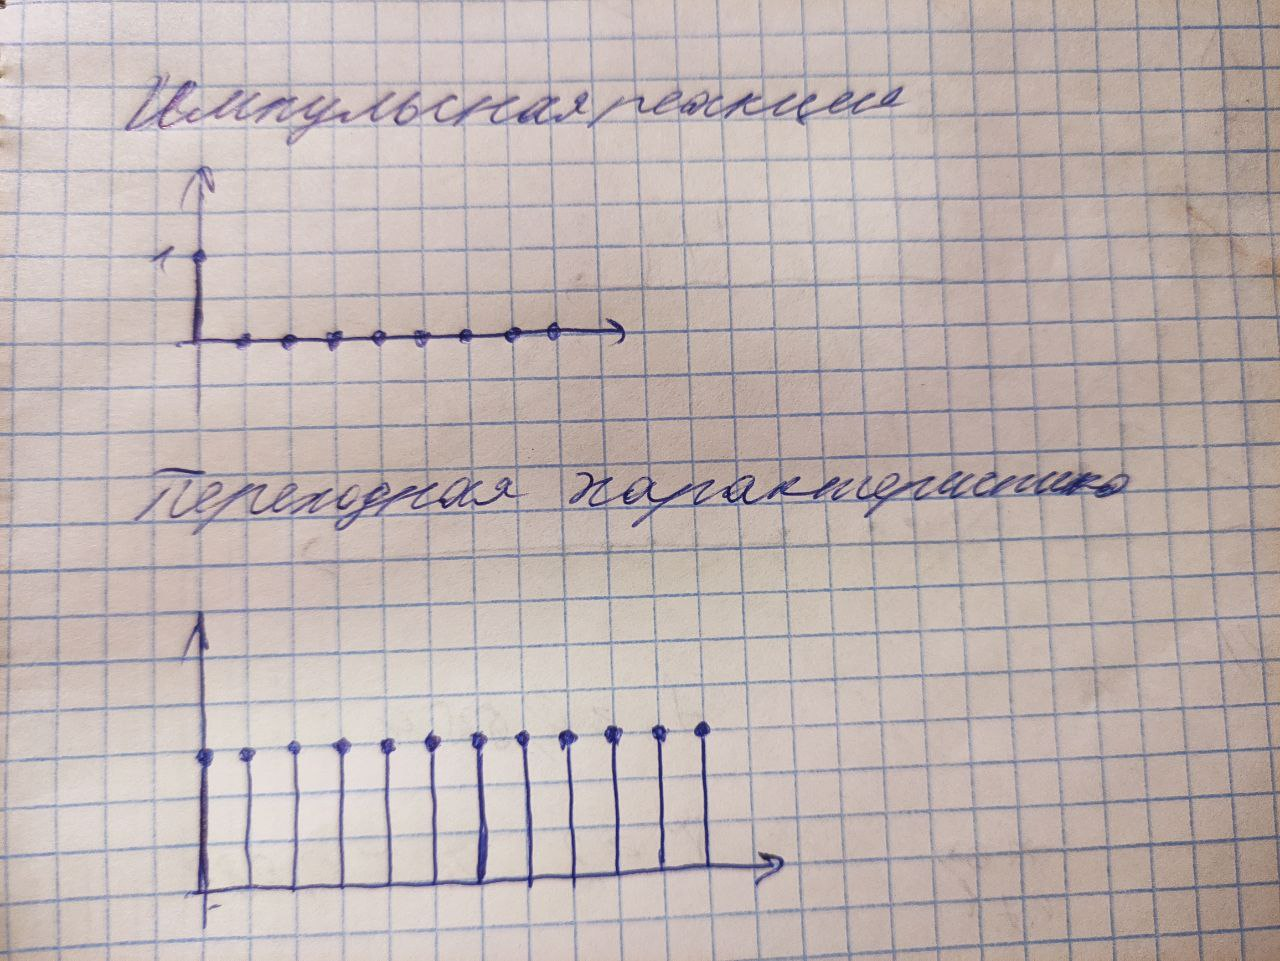
\includegraphics[scale=0.2]{images/1.7.jpg}
\caption{Импульсная реакция и переходная характеристика}
\label{1.7}
\end{figure}

\item Реализуем дифференцирующее звено с полюсом $\mu = 0.7$. Измерим верхнюю граничную частоту по уровню $-3 dB \rightarrow f_0 = 0.054$ и время спада $\tau = 3$. Видим, что формула $f_0 = \frac{1}{2\pi \tau}$ выполняется. Исследуем изменение временных и частотных характеристик при $\mu \rightarrow 0$. Изучим осциллограммы временных характеристик для двух значений $\mu$ (рис. 2).

\begin{figure}[h!]
\centering
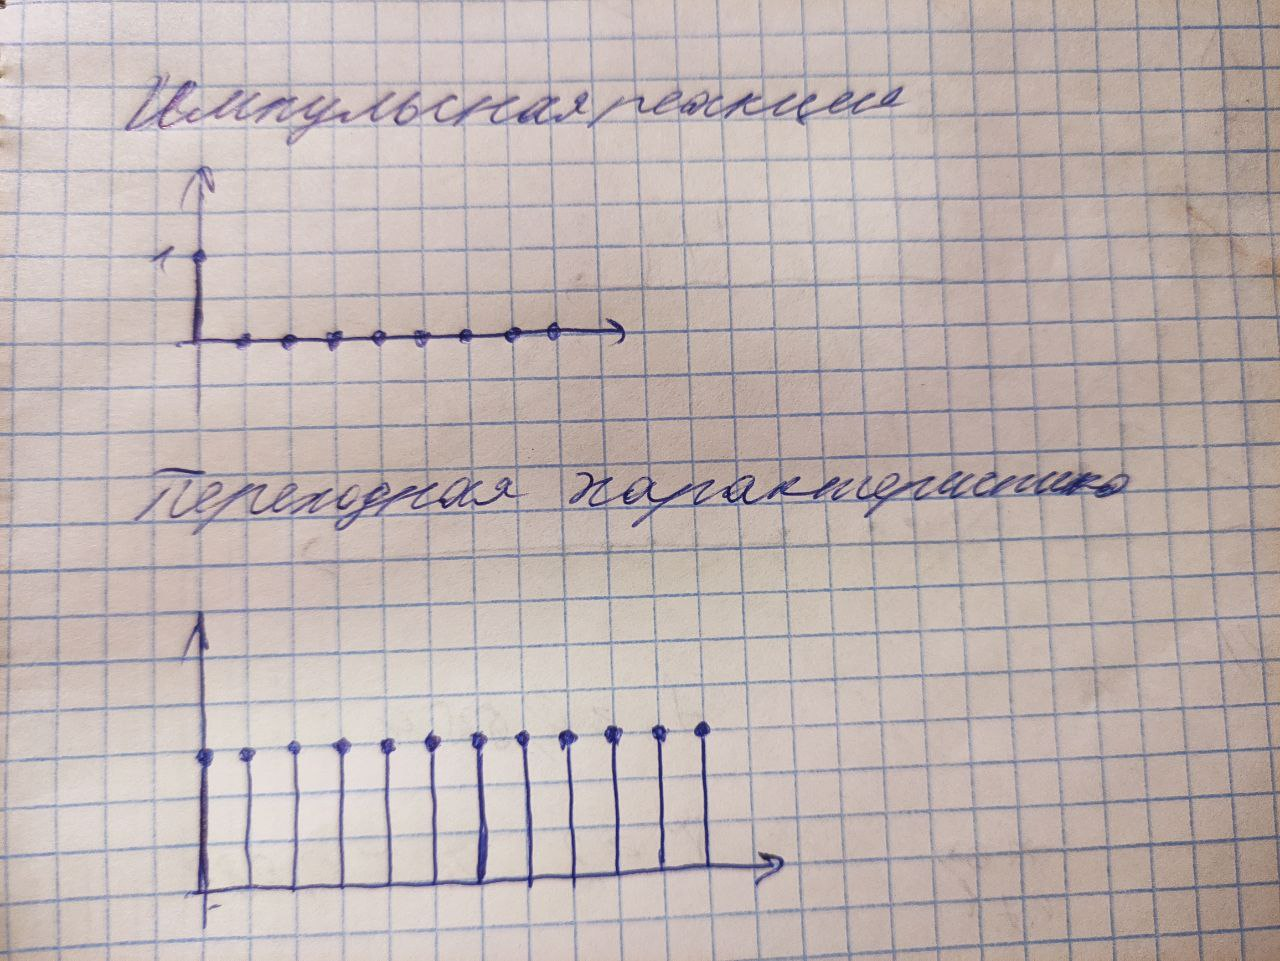
\includegraphics[scale=0.2]{images/1.7.jpg}
\caption{Осциллограммы временных характеристик для двух значений $\mu$}
\label{1.8}
\end{figure}

\newpage

\item Реализуем цифровой фазовращатель - звено:

\[H(x) = \frac{-\mu + x}{1 - \mu x} \Leftrightarrow H(z) = \frac{1 - \mu z}{z - \mu},\]

с полюсом $\mu$ и нулем $\frac{1}{\mu}$. Равномерность частотной характеристики возникает из-за того, что произведения расстояний до всех нулей и произведение расстояний для всех полюсов от точек на единичной окружности одинаковы. ФЧХ при стремлении $\mu$ к нулю представляет собой равномерно убывающую линейную функцию с уровнем $-3 dB$ на $\frac{9}{10} \frac{\pi}{2}$
\end{enumerate}

\subsection{Звенья второго порядка}

\begin{enumerate}
\item Реализуем полосовое звено с $r_{\mu} = 0.9$ и $\varphi_{\mu} = \frac{\pi}{4}$. Оценим резонансную частоту и двухстороннюю полосу пропускания по уровню $-3 dB$:

\[f_0 \simeq 0.25 \quad \bigtriangleup f = 0.067\]

В таком случае эквивалентная добротность:

\[Q = \frac{f_0}{\bigtriangleup f} = 3.73\]

\item Изучим зависимость характеристик фильтра от $r_{\mu}$ приближая его к единице:

\begin{figure}[h!]
\centering
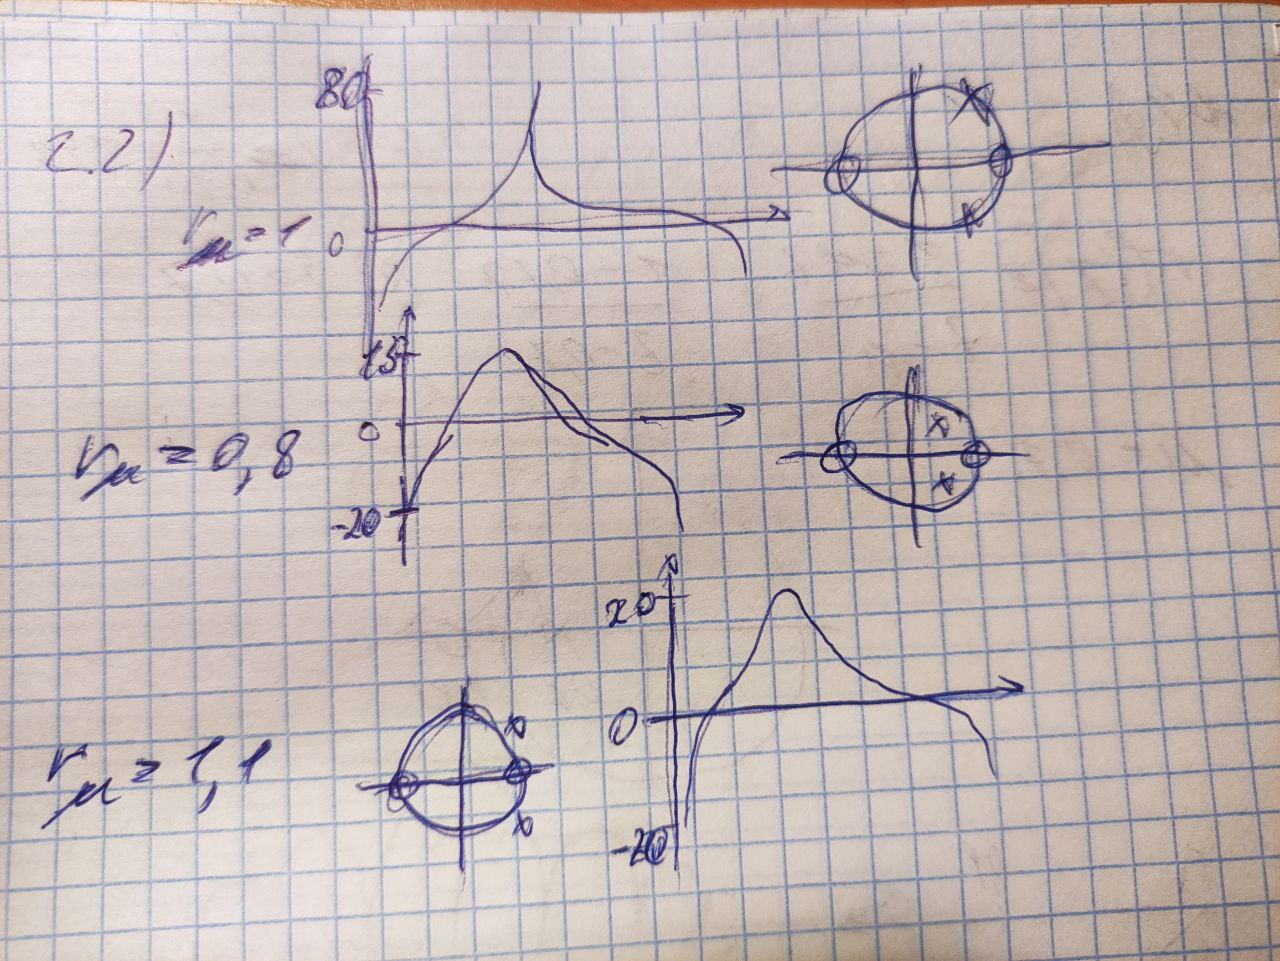
\includegraphics[scale=0.2]{images/2.2.jpg}
\caption{Зависимость характеристик фильтра от $r_{\mu}$}
\label{2.2}
\end{figure}

\item Реализуем фильтр с парой сопряженных лучей $g = [1 - r_{\nu} \cdot (2 cos \varphi_{\nu}) r_{\nu}^2]$. Изучим последствия изменения $r_{\nu}$ от 0.5 до 4 при $2 cos \varphi_{\nu} = \sqrt{2}$ и последствия изменения угла $2 cos \varphi_{\nu} = 1, \sqrt{2}, \sqrt{3}, -1, -\sqrt{2}, -\sqrt{3}$.

\item Подтвердим, что звено с $r_{\mu} = 0.8$ и $r_{\nu} = \frac{1}{r_{\mu}} = 1.25$ является \textit{all pass} фильтром с равномерной частотной характеристикой при любых одинаковых $\varphi_{\mu}, \varphi_{\nu}$.
\end{enumerate}

\subsection{Нерекурсивные FIR фильтры}

\begin{enumerate}
\item Реализуем гребенчатый фильтр порядка $N = 3$ с $H(x) = 1 - x^3$. Заметим, что при увеличении порядка фильтра увеличивается количество пиков.

\item Реализуем фильтр порядка $N = 7$ с прямоугольной импульсной реакцией: $h = [1 1 1 1 1 1 1 1], g = [1]$. Измерим все четыре пиковые значения коэффициента передач:

\[K_1 = 18.1 dB \quad K_2 = 5.27 dB \quad K_3 = 1.63 \quad K_4 = 0.18 dB\]

Убедились, что эти уровни не зависят от порядка $N$, и что тот же фильтр дают настройки $h = [1 0 0 0 0 0 0 0, -1], g = [1 -1]$. Посмотрим на временную характеристику (рис. 4).

\begin{figure}[h!]
\centering
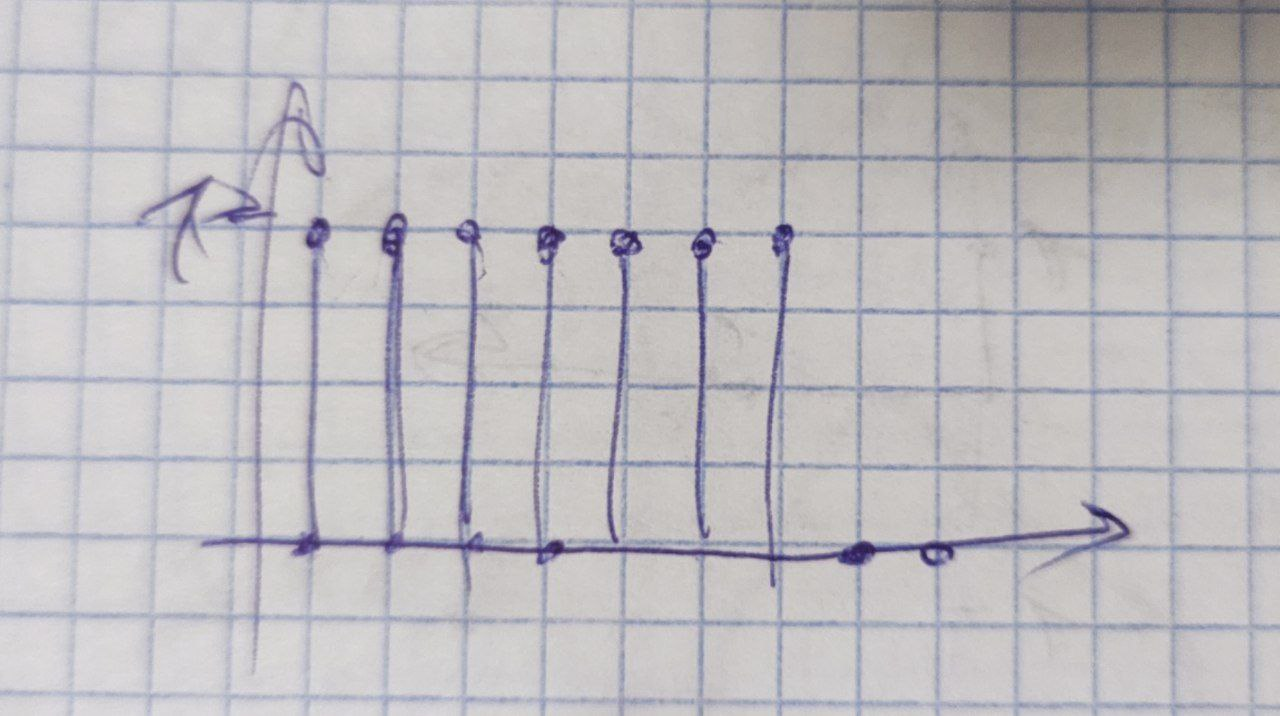
\includegraphics[scale=0.2]{images/3.2.jpg}
\caption{Временная характеристика}
\label{2.2}
\end{figure}

\item Организуем децимацию выхода этого фильтра по индексу D = 4 (рис. 5). Повторим это для фильтра $h = [1 1 1 1]$ (рис. 6). На рисунках сверху показан спектр после децимации, а снизу до.

\begin{figure}[h!]
        \begin{center}
            \begin{minipage}[h!]{0.48\linewidth}
                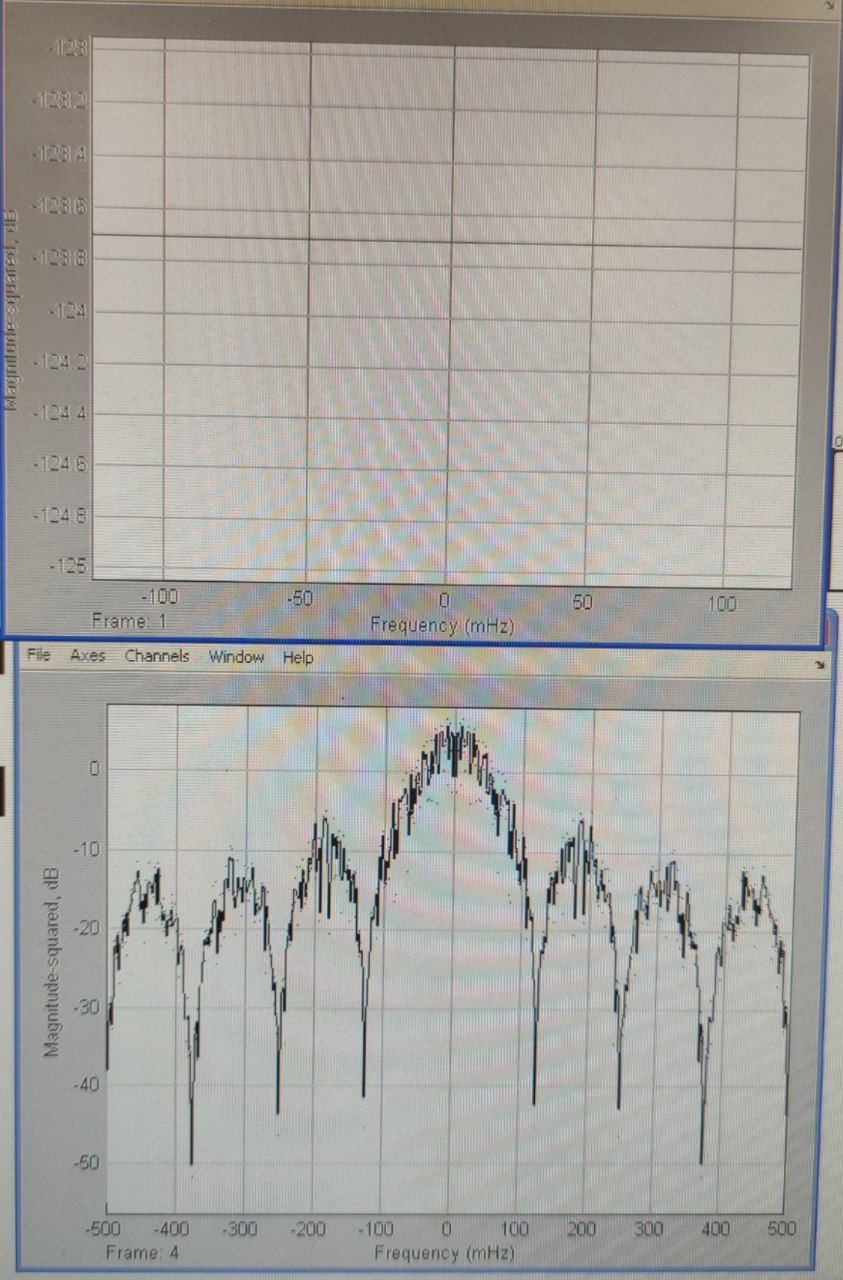
\includegraphics[width=1\linewidth]{images/3.3_1.jpg}
                \caption{Фильтр $h = [1 1 1 1 1 1 1 1], g = [1]$}
                \label{picture_2}
            \end{minipage}
            \hfill
            \begin{minipage}[h!]{0.48\linewidth}
                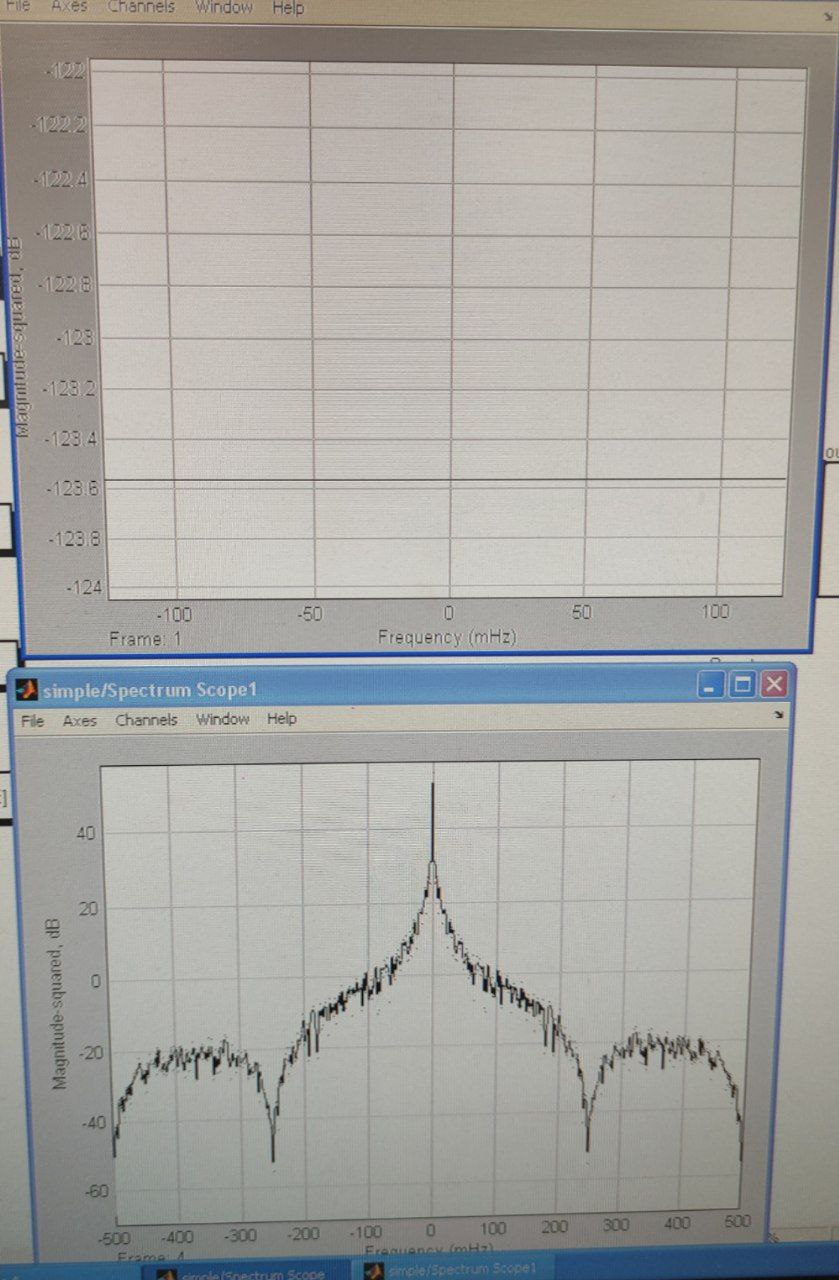
\includegraphics[width=1\linewidth]{images/3.3_2.jpg}
                \caption{Фильтр $h = [1 1 1 1]$}
                \label{picture_3}
            \end{minipage}
        \end{center}
    \end{figure} 
    
\newpage

\item Подадим на вход гармонический сигнал частоты 0.126/2. Оценим коэффициент передачи:

\[K \simeq 10\]

Запомним амплитуду и временную форму сигнала после децимации (D = 4). То же самое сделаем для сигналов при входных частотах $0.5/2 \pm 0.126/2$ и $1/2 \pm 0.126/2$:

\[2A = 18 \quad K \simeq 10\]

\[2A = 1 \quad K = 0.5\]

\[2A = 0.8 \quad K = 0.4\]

\item Изучим фильтры с временными окнами. Сравним характеристики оконных фильтров порядка $2N + 1 = 41$ с различными типами окон, измерив для каждого и них полуширину главного пика, уровень затухания в главном и побочном пиках:

\begin{center}
\begin{tabular}{|c|c|c|}
\hline 
 & Главный & Побочный \\ 
\hline 
Полуширина & 0.025 & 0.024 \\ 
\hline 
Уровень затухания & 0 dB & -13.3 dB \\ 
\hline 
\end{tabular} 
\end{center}

Сделаем то же самое для $N = 40$:

\begin{center}
\begin{tabular}{|c|c|c|}
\hline 
 & Главный & Побочный \\ 
\hline 
Полуширина & 0.012 & 0.012 \\ 
\hline 
Уровень затухания & 0 dB & -13.4 dB \\ 
\hline 
\end{tabular} 
\end{center}

\item Изучим фильтры с частными окнами. Реализуем фильтр с полосой в половину полосы Найквиста, набрав в поле \textit{Numerator coefficients} fwdw(20,10,10). Измерим затухание в первом побочном пике и на границе полосы Найквиста. Повторим эти измерения изменяя интервал сглаживания - $k = 8, 6, 4, 2, 0$ (fwdw(N,k,n)):

\begin{center}
\begin{tabular}{|c|c|c|}
\hline 
k & Главный пик, dB & Побочный пик, dB \\ 
\hline 
10 & -16.3 & -29.1 \\ 
\hline 
8 & -21.9 & -37.3 \\ 
\hline 
6 & -28 & -43.5 \\ 
\hline 
4 & -31.6 & -47 \\ 
\hline 
2 & -34.1 & -49.6 \\ 
\hline 
0 & -36 & -51.5 \\ 
\hline 
\end{tabular} 
\end{center}

\item Увеличивая порядок N, синтезируем фильтр с $k = \frac{N}{4}, n = \frac{N}{2}$, который обеспечивает затухание 80 dB в дальней зоне - N = 160.

\item Откроем модель 4-звенного CIC-фильтра из блоков IC с задержкой N = 12. Изучим временные (PULSE, STEP) и частотные (CHIRP) характеристики блоков и фильтра в целом (рис. 7, 8, 9).

\begin{figure}[h!]
        \begin{center}
            \begin{minipage}[h!]{0.32\linewidth}
                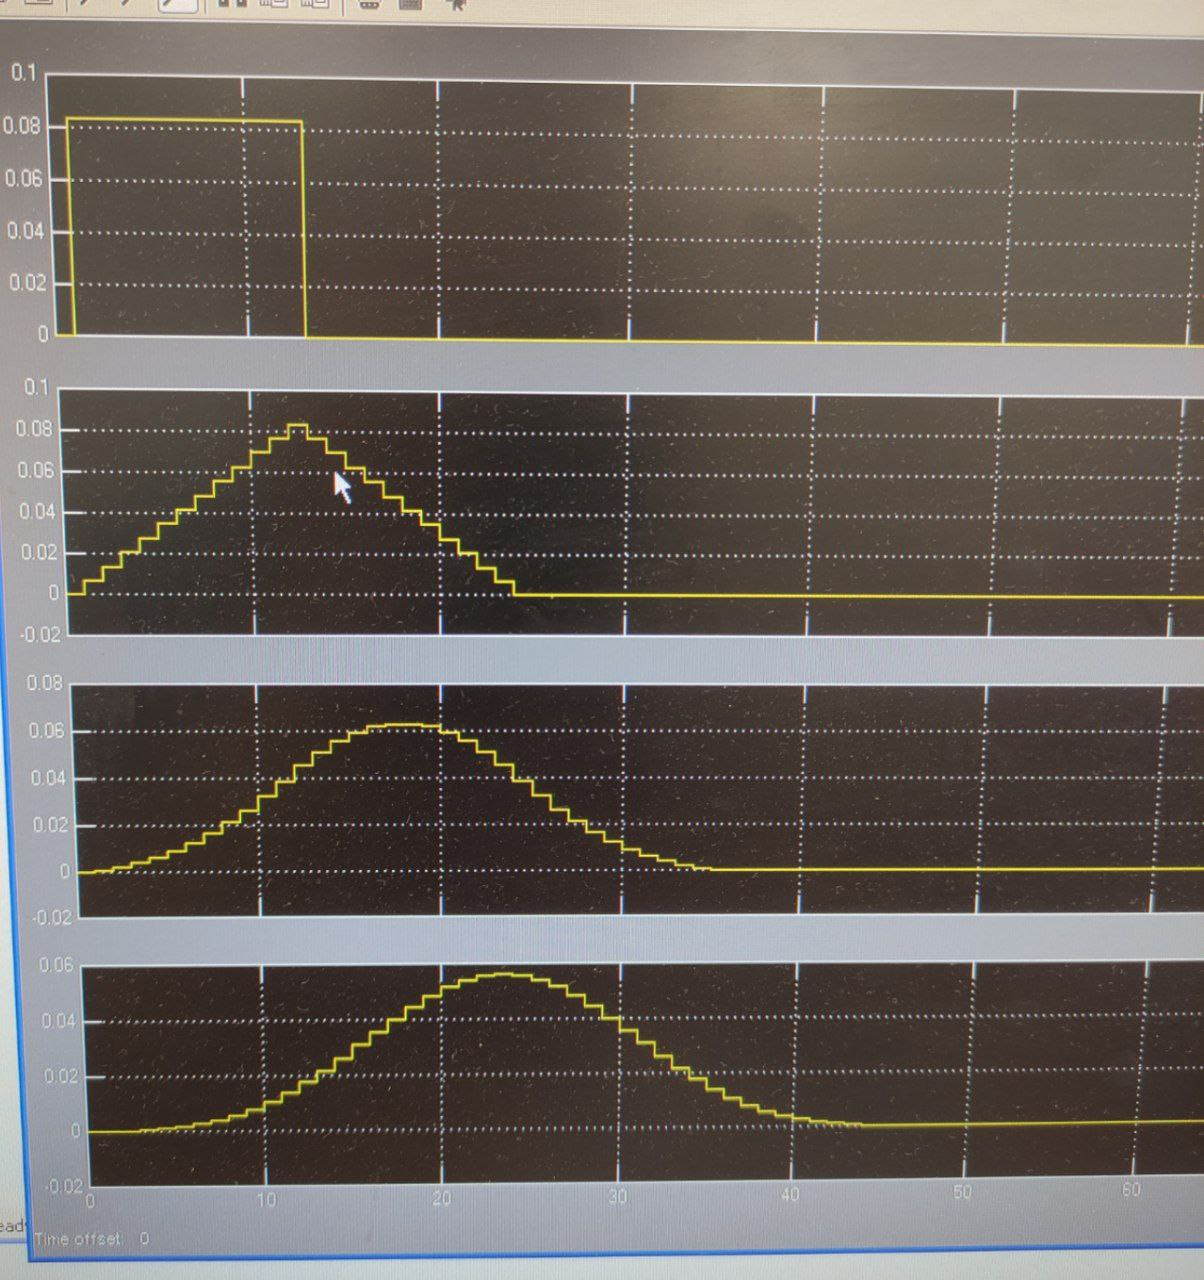
\includegraphics[width=1\linewidth]{images/3.7_1.jpg}
                \caption{Временные характеристики (PULSE)}
                \label{3.7_1}
            \end{minipage}
            \hfill
            \begin{minipage}[h!]{0.32\linewidth}
                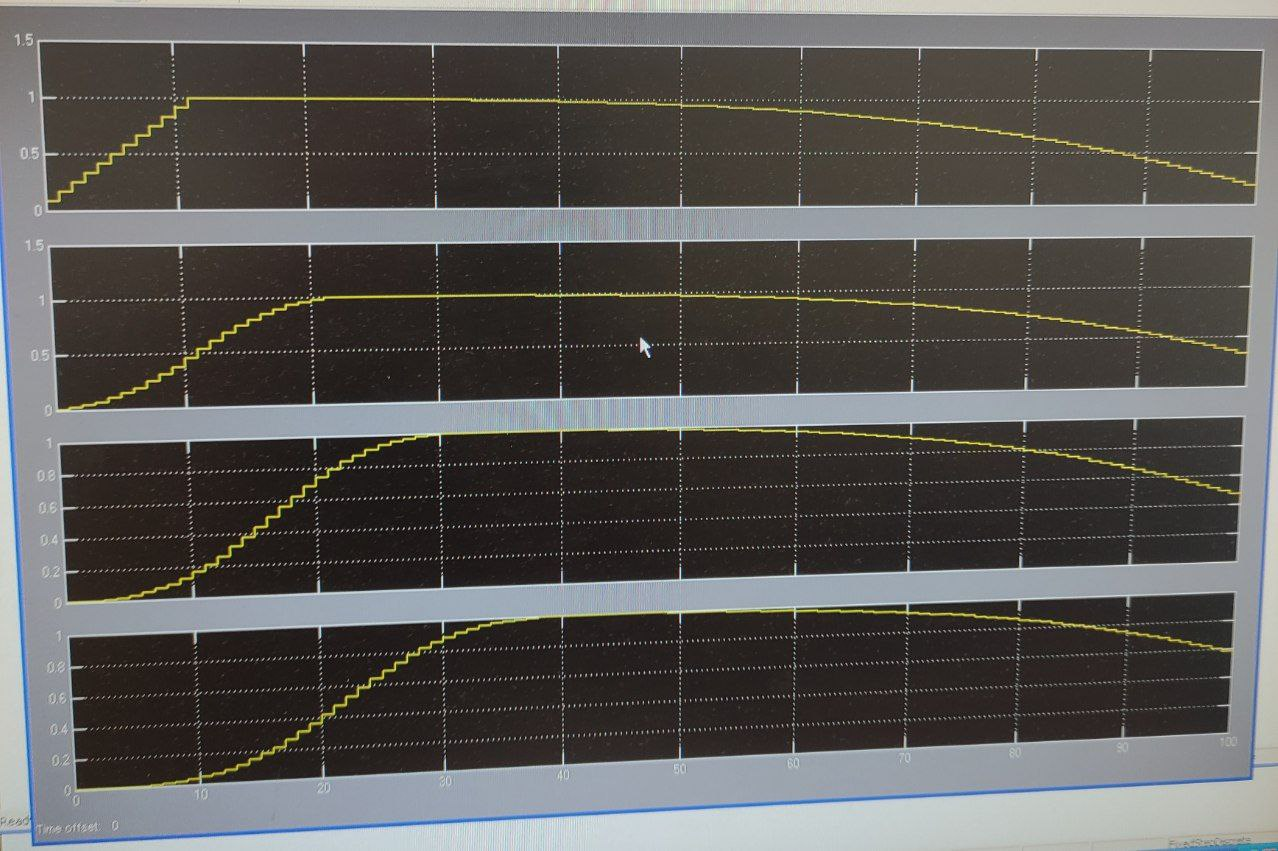
\includegraphics[width=1\linewidth]{images/3.7_2.jpg}
                \caption{Временные характеристики (STEP)}
                \label{3.7_1}
            \end{minipage}
            \hfill
            \begin{minipage}[h!]{0.32\linewidth}
                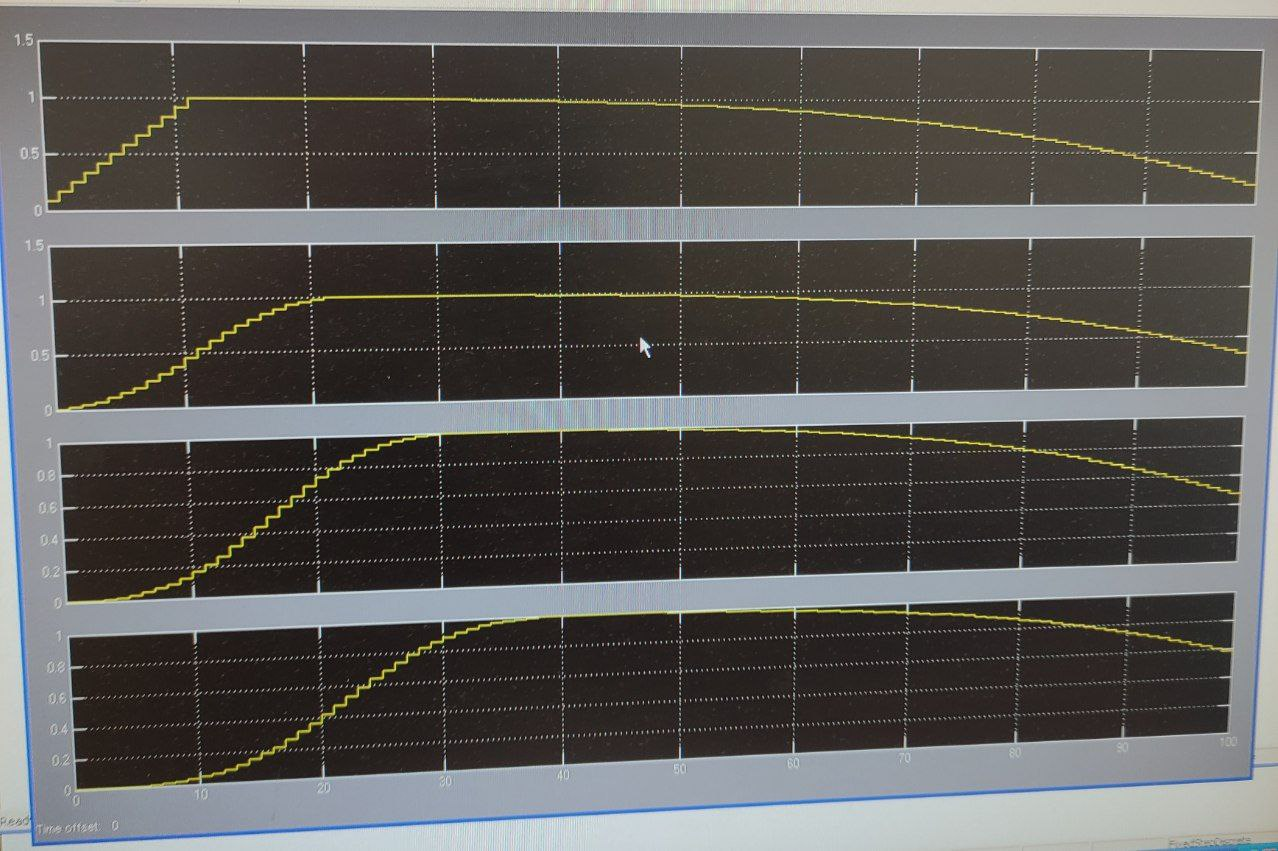
\includegraphics[width=1\linewidth]{images/3.7_2.jpg}
                \caption{Частотные характеристики (CHIRP)}
                \label{3.7_3}
            \end{minipage}
        \end{center}
    \end{figure}
    
По графику спектральной плотности шума оценим ширину главного пика и уровни затухания в первых побочных пиках и пиках вблизи границы полосы Найквиста:

\begin{center}
\begin{tabular}{|c|c|c|c|}
\hline 
 & Главный пик & Побочный пика & На границе \\ 
\hline 
Ширина полосы & 85 & 37.5 & -- \\ 
\hline 
Уровень затухания & -15 dB & -65 dB & -100 dB \\ 
\hline 
\end{tabular} 
\end{center}

Сравнив уровни сигнала на выходе дециматора при частотах $a_1 = 1.01/24$ и $a_2 = 1/6 \pm 1.01/24$:

\[K_{a_1} = 0.17 \quad K_{a_2} = 3 \cdot 10^{-4}\]
\end{enumerate}

\subsection{FDATool Matlab}

\begin{enumerate}
\item Изучим синтезатор \textit{equiripple} FIR-фильтров. Синтезируем фильтр минимального порядка с \textit{wpass} = 0.4, \textit{wstop} = 0.5, \textit{Apass} = 1, \textit{Astop} = 60.

\item Изучим синтезатор типовых IIR-фильтров - Баттерворта, Чебышева типов I и II и эллиптических. Синтезируем фильтры с параметрами \textit{wpass} = 0.4, \textit{wstop} = 0.5, \textit{Apass} = 1, \textit{Astop} = 60, изучим результаты.

\item Синтезируем FIR фильтр с характеристиками \textit{wpass} = 0.3, \textit{wstop} = 0.5, \textit{Apass} = 1, \textit{Astop} = 80 b и все четыре варианта IIR фильтров с теми же характеристиками. Запишем количество нулей у каждого фильтра:

\begin{center}
\begin{tabular}{|c|c|}
\hline 
Имя фильтра & Количество нулей \\ 
\hline 
Equiripple & 25 \\ 
\hline 
Butterworth & 15 \\ 
\hline 
Chebyshev I & 9 \\ 
\hline 
Chebyshev II & 9 \\ 
\hline 
Elliptic & 6 \\ 
\hline 
\end{tabular} 
\end{center}

Заметим, что нам легче синтезировать фильтр с меньшим количеством нулей.
\end{enumerate}

\section{Вывод}

В ходе данной работы мы научились пользоваться Matlab Simulink. Изучили фильтры первого и второго порядка, посмотрели как они влияют на различного вила сигналы. Узнали, что такое децимация сигнала. Изучили нерекусивные FIR-фильтры. Изучили синтезатор IIR и FIR фильтров. На примере увидели преимущества IIR решений по сравнению с FIR.


%Вставка изображения
%\begin{figure}[h!]
%\centering
%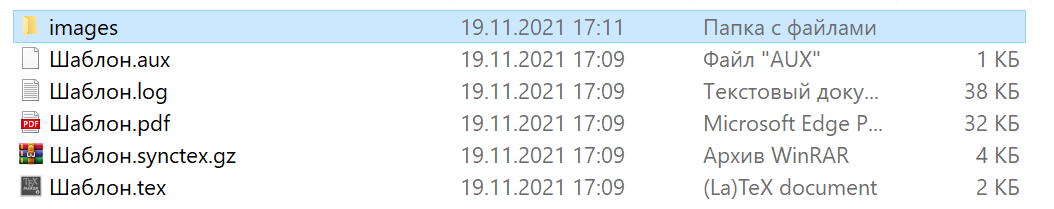
\includegraphics[scale=1]{images/image.png}
%\caption{text}
%\label{fig:Image1}
%\end{figure}


\end{document}